\small
\frame
{
	\frametitle{院士工作站计划设想}
	\begin{itemize}
		\item 材料``多学科集成''设计与计算基础课程
			\begin{itemize}
				\item 材料设计与新材料发展
				\item 计算材料与基本算法
				\item 高温合金材料学基础与相关物性机制
				\item 计算材料学中的物理化学计算技术
				\item 计算理论基础及程序分析
			\end{itemize}
		\item 材料基本物性调控与新材料探索
			\begin{itemize}
				\item 高温合金材料的物性与制备:~资深四代高温合金研究
				\item 材料固体断裂解析表示和\textrm{Griffith}断裂理论
				\item 探索航天材料:~高超音速材料
			\end{itemize}
	\end{itemize}
}

\frame[allowframebreaks]
{
	\frametitle{关于材料``多学科集成''课程的建议}
	\begin{itemize}
		\item \textcolor{magenta}{拓宽视野}\\
			物质科学研究的技术手段日益丰富:~材料基因组基本思想
\begin{figure}[h!]
\vspace*{-0.08in}
\centering
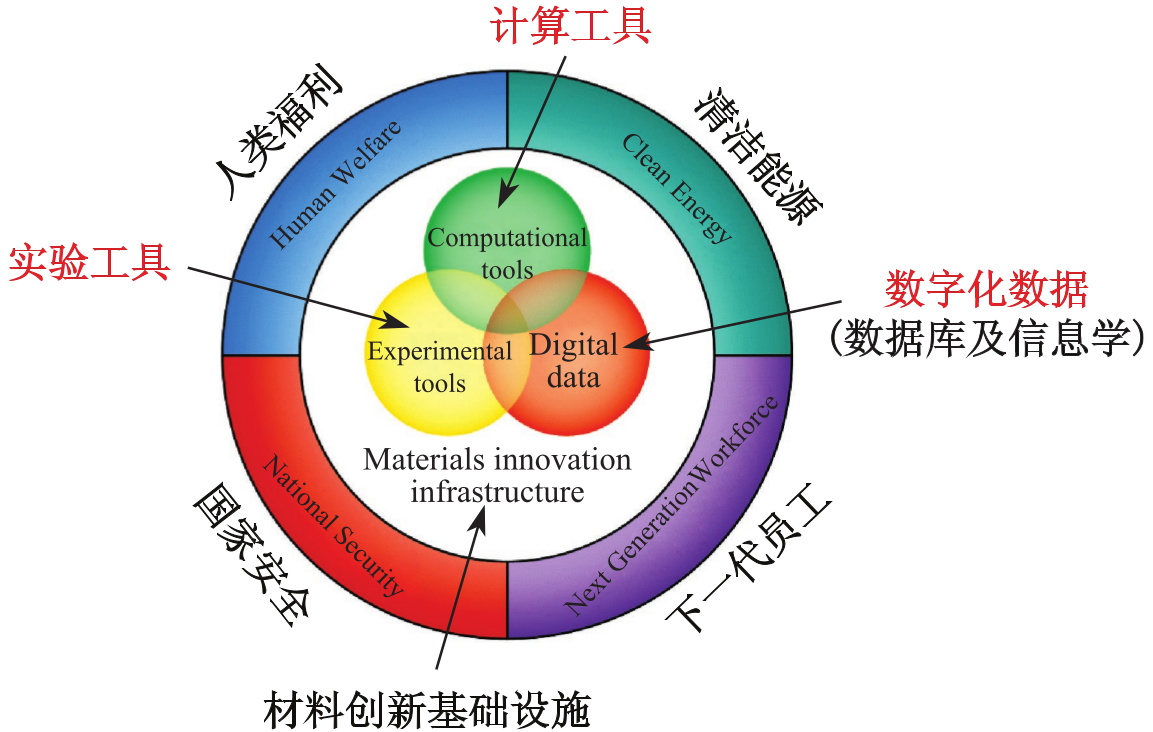
\includegraphics[height=1.55in,width=2.35in]{Figures/MGE.png}
\label{MGE}
\end{figure}
			理论计算方法多样性:~第一原理计算-分子动力学-有限元结构力学方法
		\item \textcolor{magenta}{加强基础}\\
			\begin{itemize}
				\setlength{\itemsep}{8pt} 
				\item 计算物理学的基本思想
				\item 密度泛函理论和分子动力学模拟的基本思想与应用
				\item 计算理论基础与程序\\
已编撰相应的教材和讲义
\begin{figure}[h!]
\centering
\hspace*{-0.30in}
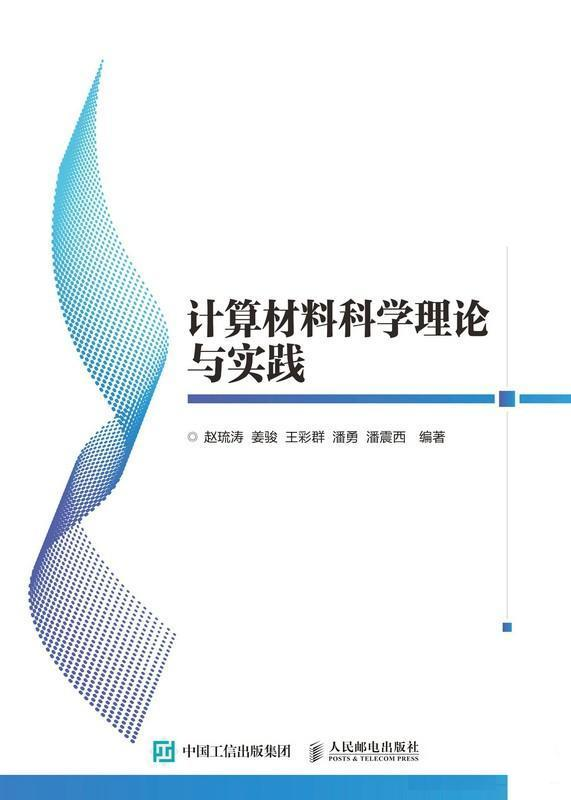
\includegraphics[height=1.45in,width=1.15in]{Figures/Computing_Materials.jpg}
\hspace{0.05pt}
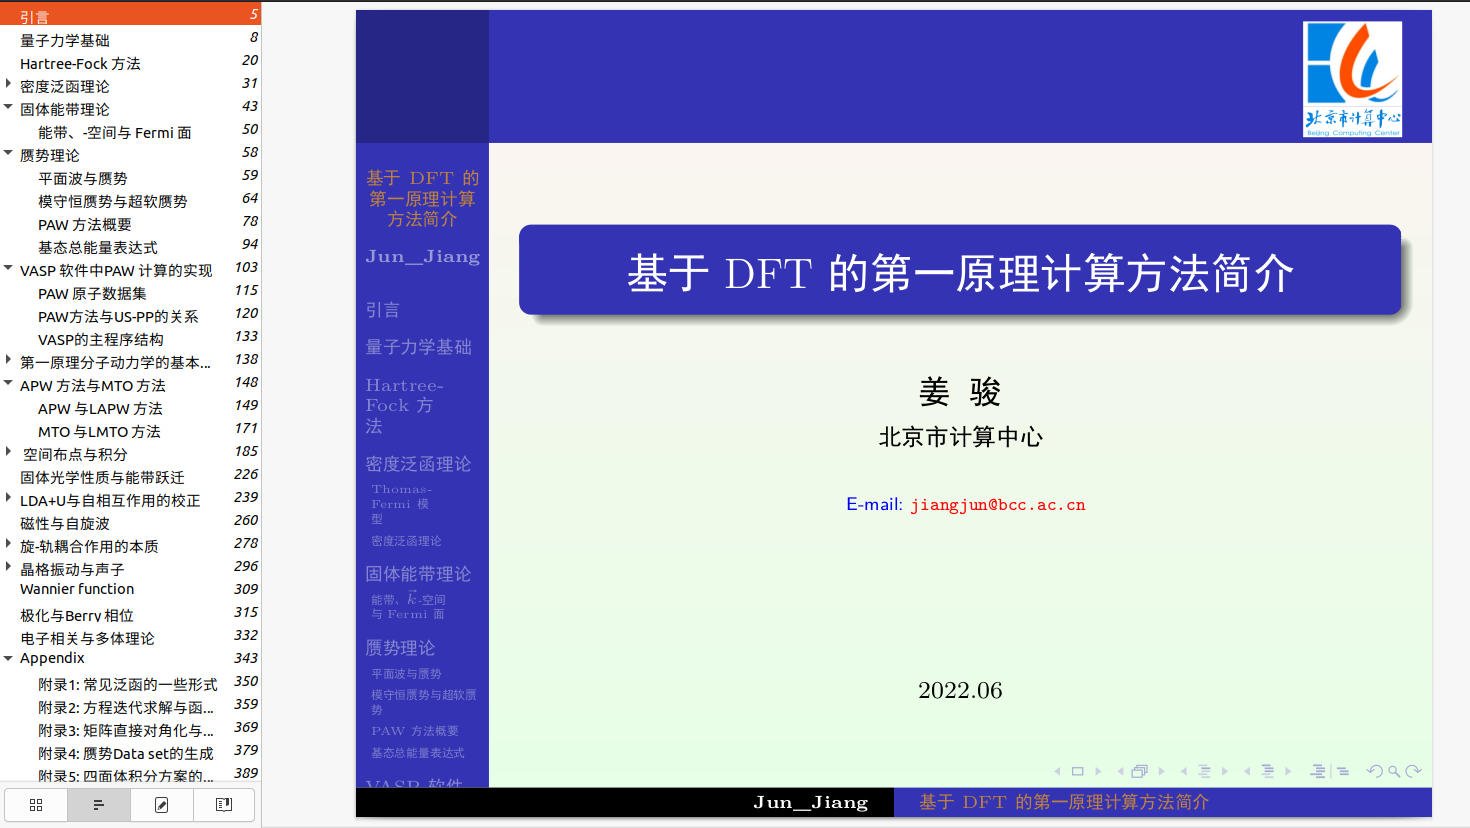
\includegraphics[height=1.45in,width=2.40in]{Figures/DFT-total.png}
\label{TEXT_PPT}
\end{figure}
	\end{itemize}
		\item \textcolor{magenta}{学科交叉}:~ 强化高温合金材料学基础
			\begin{itemize}
				\setlength{\itemsep}{3pt} 
		\item 多尺度跨层次计算
\begin{figure}[h!]
\vspace*{-0.02in}
\centering
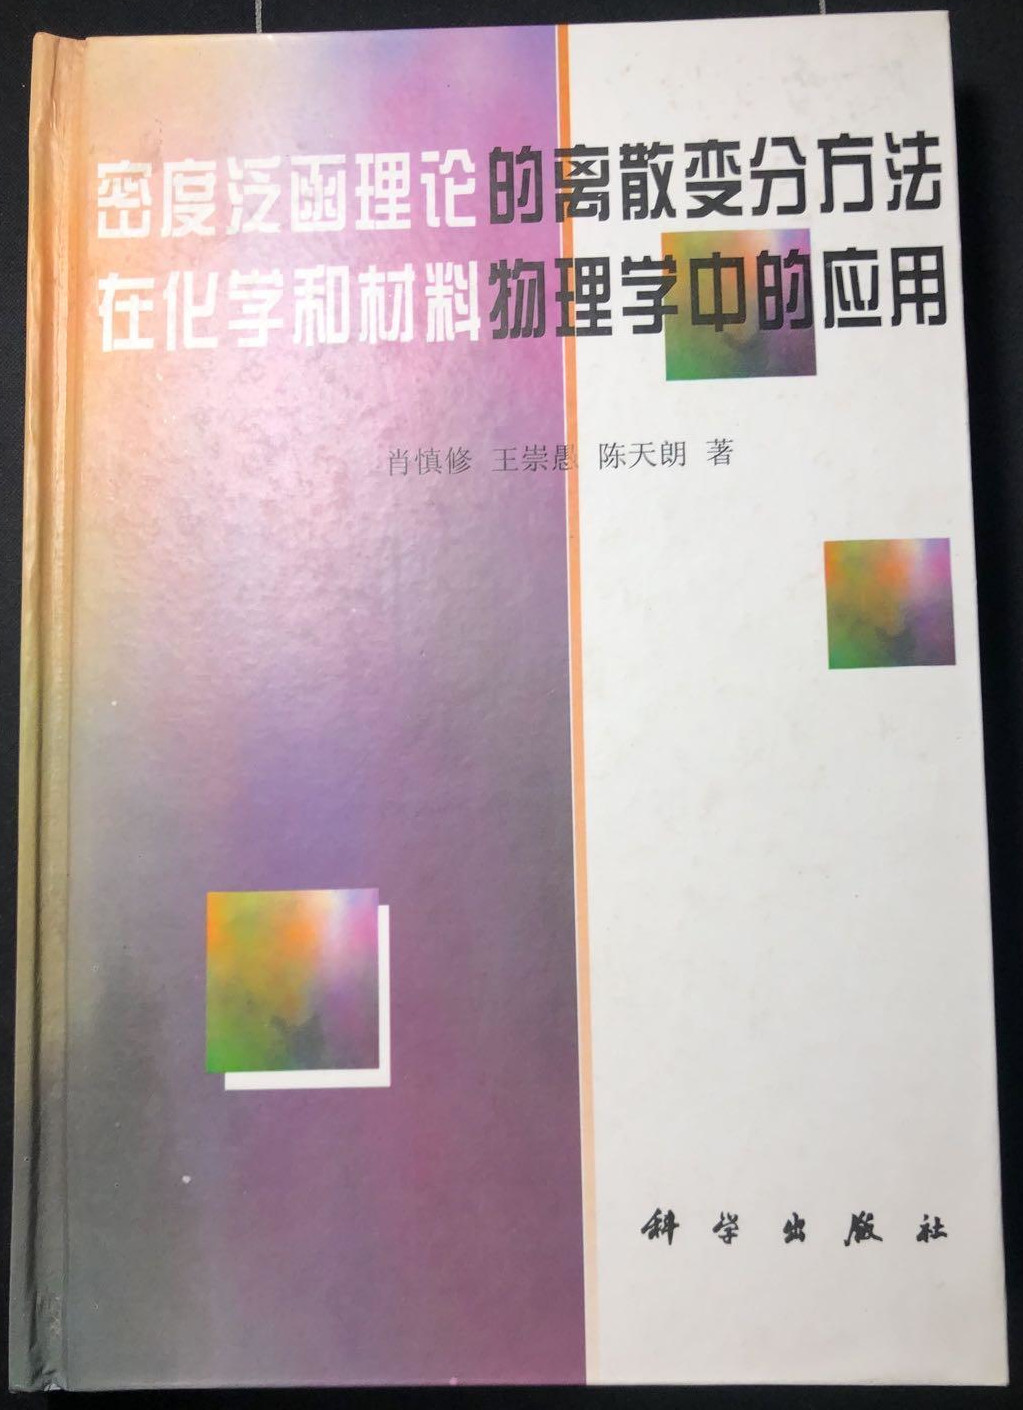
\includegraphics[height=1.55in,width=1.15in]{Figures/DFT_Wang.jpg}
\label{DFT_Wang}
\end{figure}
		 \item 结构材料的化学组元与占位\\
			配位场与化学键理论
		 \item 计算材料学中的物理化学计算技术
	\end{itemize}
\end{itemize}
}

\frame[allowframebreaks]
{
	\frametitle{关于材料基本物性调控与新材料研究的建议}
	\begin{itemize}
				\setlength{\itemsep}{8pt} 
				\item \textcolor{blue}{高温合金材料研究}\\
			航空发动机是高温合金材料的重要应用领域,是飞机的心脏\\
			单晶叶片是航空发动机的核心部件,工作温度高达1800$^{\circ}\mathrm{C}$\\
			高温合金研发成本高昂,发展高通量多尺度并发式集成计算算法和相应的软件系统为基础,有望提升资深资源化高温合金的性能和降低成本
\begin{figure}[h!]
\vspace*{-0.02in}
\centering
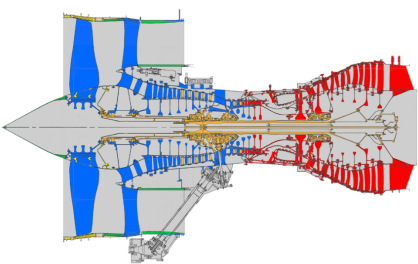
\includegraphics[height=1.25in,width=1.55in]{Figures/Engineering_1.png}
\hspace{0.01pt}
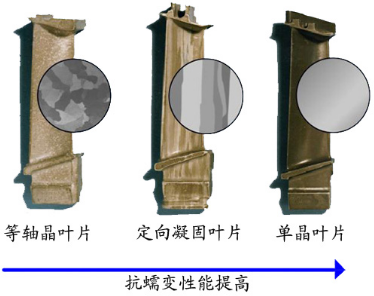
\includegraphics[height=1.25in,width=1.65in]{Figures/Engineering_2.png}
\label{Engineering}
\end{figure}
%研发国家重大需求的资源化高温合金为驱动和牵引
		\item \textcolor{blue}{高超音速材料研究}\\
高超音速技术领域目前是航空航天及国防工业的热门话题,高超音速飞行器采用超音速冲压发动机,主要包括:
\begin{itemize}
	\item 高超音速巡航导弹
	\item 高超音速飞机
	\item 航天飞机
\end{itemize}
美国正大力发展高超音速武器,根据美国军方公开的报道,至少有5中不同的高超音速武器项目正处于开发中\\
\textcolor{purple}{纳米技术}正成为研制高超音速武器的一项关键技术,其最新的发展能够使导弹平台以超过5倍音速的速度在大气层中运行,其中碳纳米管方面的突破使其有望成为一种强度高、重量轻且能够迅速散热的适用性新材料\\
中美俄在高超声速武器的研究项目上竞争激烈,关键在于两个方面:~研发出耐高温的材料和超燃冲压发动机,\textcolor{red}{耐高温材料是关键中的关键}
\begin{figure}[h!]
\vspace*{-0.20in}
\centering
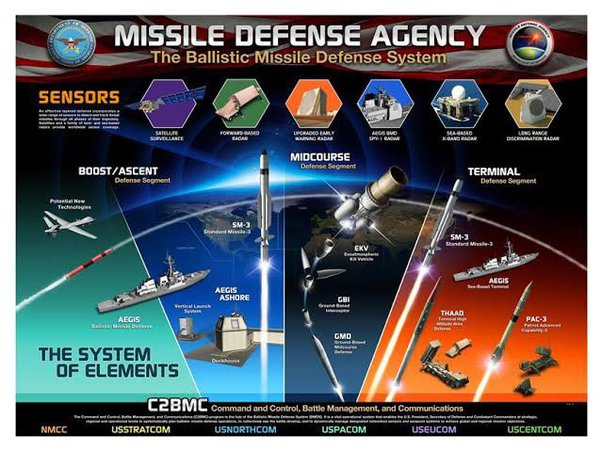
\includegraphics[height=2.90in,width=3.70in]{Figures/Main-qimg.jpeg}
\label{BMDS}
\end{figure}
	\end{itemize}
}
